	
\tab The classes in the model package are designed to hold all the relevant data about a document. When saving files, the model is all that is saved and it is all that is necessary to then completely reconstruct the whole document. A document, that is a user-created class diagram, is represented by the DocumentModel class. 

\paragraph{\small{\tab DocumentModel and DocumentPreferences\\*}}

\hspace{-10pt}This class acts mainly as a wrapper for all the data about a document. By passing a DocumentModel object around, we can pass the whole of the model.  The class holds a DocumentPreferences object that stores persistent global data about a document like font, canvas size, associated filename and zoom. The DocumentPreferences class extends Observable which lets individual model elements react to changes the user makes to it by acting as Observers. The second principal data field in DocumentModel is an ArrayList of DocumentElementModels.

\newpage
% 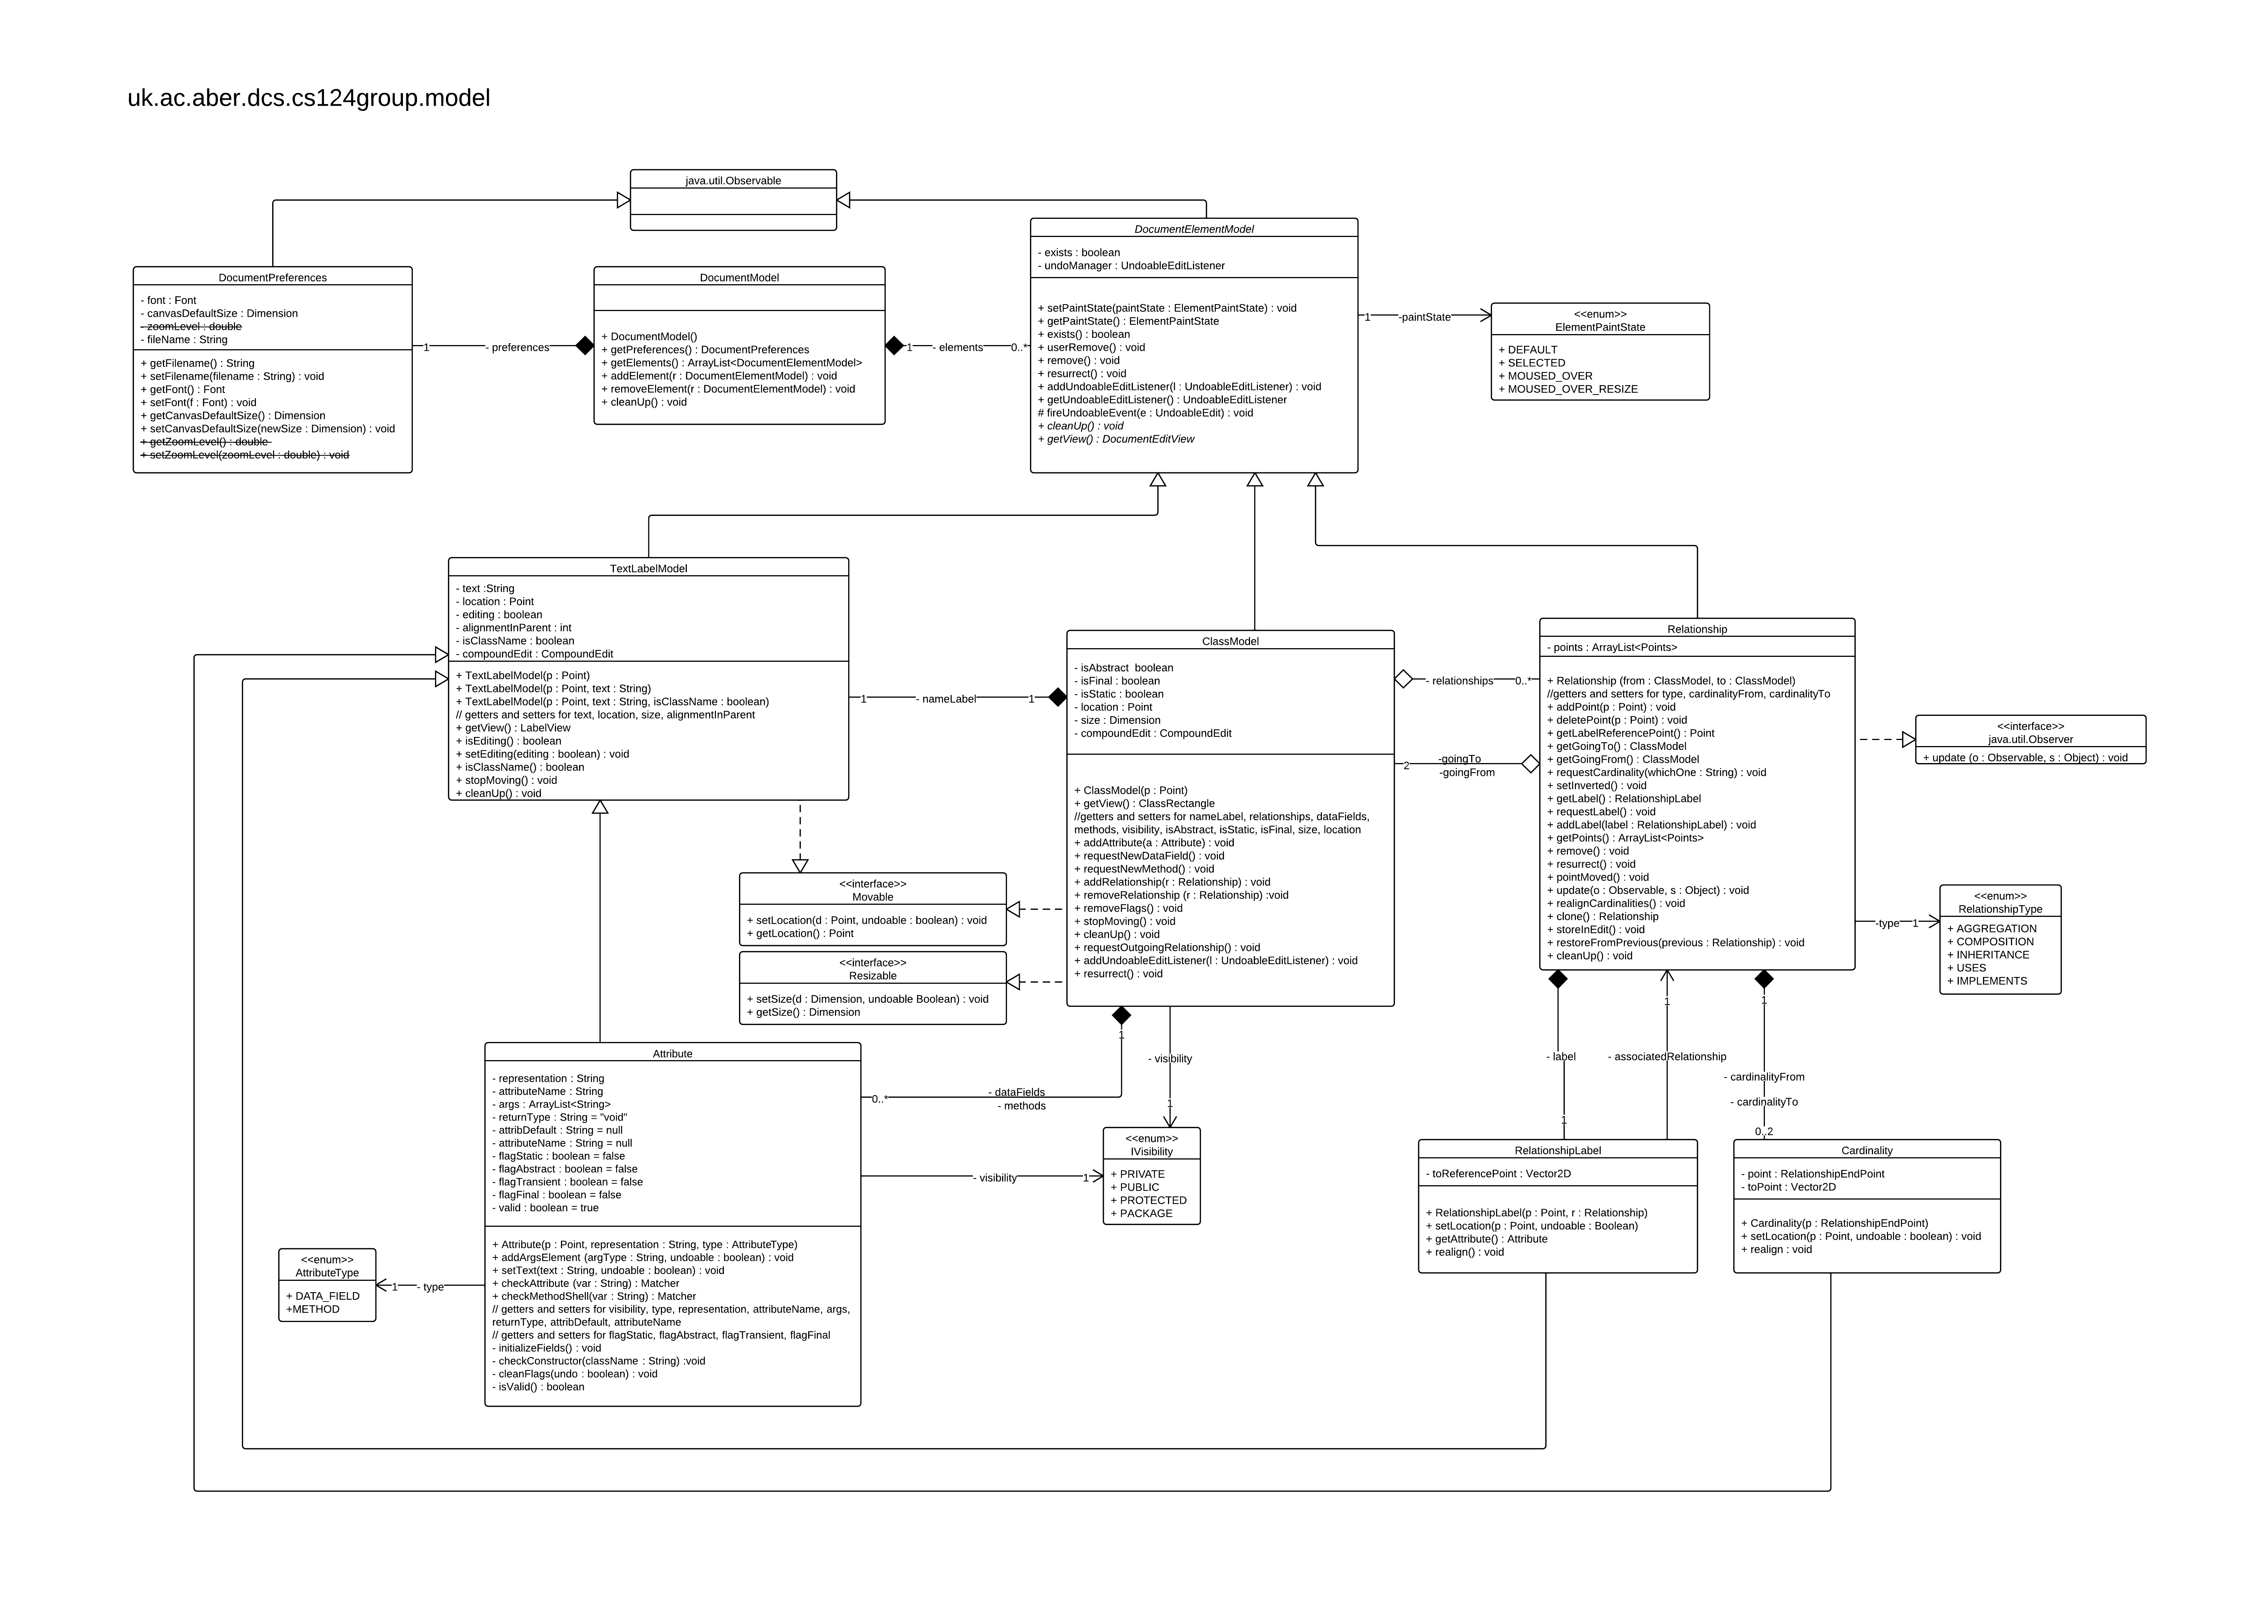
\includepdf{modelClassDiagram.pdf}
\newpage

\paragraph{\small{\tab DocumentElementModel and ElementPaintState\\*}}

\hspace{-10pt}An 'element' is understood to be a discrete, controllable and viewable entity in the class diagram. All elements the application supports share a certain amount of characteristics. These are represented in the abstract DocumentElementModel class. The most important characteristic is existence (this includes the remove() and resurrect() methods). More information about what this means and how existence is handled within the application, please refer to section X.X on undos. Other characteristics shared by elements are, font, zoom and the paint state. The enum ElementPaintState defines four possible states an element may be in based on mouse actions. This is used not only to work out exactly how an element is to be painted but can also be used to find out when an element has been clicked on from outside its own MVC triad. The other fields and methods in DocumentElementModel relate to the undo functionality, described in section X.X.

\paragraph{\small{\tab Textual elements: TextLabelModel, Attribute, Cardinality, RelationshipLabel\\*}}

\hspace{-10pt}Any textual element in the class diagram is actually a text label, represented by a TextLabelModel object. It can either be a plain label sitting somewhere outside any other element or it can be a class name, an attribute, a cardinality or a relationship label. The latter three all have their own model classes that extend TextLabelModel which defines basic operations like setting the text, location and size in the class diagram and enabling editing. Subclasses of TextLabelModel will usually restrict their own movability.

\paragraph{\small{\tab Attribute, again\\*}}

\hspace{-10px}This class merits its own section as understanding how it works is crucial to understanding the export functionality. Attributes are split into two types . data fields and methods. They have a representation . a String that the user enters into the class diagram. From this String, information is extracted about the visibility, type, default value, return type and arguments, where applicable, and attributes of this class are initialised. Modifiers can be added and edited by right-clicking. When exporting Attributes into java code, the Exporter class only looks at these initialised fields. If the representation does not conform to UML standards, the Attribute is flagged as invalid and is ignored by the Exporter. Exportable Attributes may also be obtained by calling the getAttribute() method on a RelationshipLabel object.

\paragraph{\small{\tab ClassModel\\*}}

\hspace{-10px}As the name suggests, ClassModels hold data about a class rectangle in the UML diagram. They all contain a TextLabelModel that is the name of the class shown on the top of the rectangle and may also contain user-defined Attributes and Relationships. Also provided are modifier and visibility flags. Methods for manipulating all of this data are defined in the class.

\paragraph{\small{\tab Relationship\\*}}

\hspace{-10px}Relationships represent data about .arrows. on the class diagram. They have a type, a .from. ClassModel, which is always the class at which the arrowhead or diamond is shown, regardless of the type, a .to. ClassModel and an ArrayList of user-defined points. They may also contain two Cardinalities and a RelationshipLabel. Methods manipulating all of this data are provided, as well as cloning and restoring facilities that are used by the undo functionality. 

\paragraph{\small{\tab Movable and Resizable\\*}}

\hspace{-10px} These are two interfaces implemented by user-movable and / or user-resizable elements. Currently, ClassModel implements both and TextLabelModel implements Movable. These classes are mainly defined to facilitate undo functionality.

\paragraph{\small{\tab The enums: IVisibility, RelationshipType, AttributeType\\*}}

\hspace{-10px}These are used in place of static constants and are very much self-explanatory.


